\subsection*{ĐỀ THI THỬ THPTQG SỞ GD \& ĐT NGHỆ AN 25-26, LẦN 3}
\caulc
\Opensolutionfile{ans}[ans/ans-26-2--SoGD-L1-LC]
\begin{ex}% Câu 1%[Võ Xuân Cường Thịnh]%[2D4N3-3]
	Cho hình phẳng $(H)$ giới hạn bởi các đường $y=x+2$, $y=0$, $x=0$, $x=2$. Gọi $V$ là thể tích của khối tròn xoay được tạo thành khi quay $(H)$ xung quanh trục $Ox$. Mệnh đề nào dưới đây đúng?
	\choice
	{$V=\displaystyle \int \limits_{0}^{2}(x+2)\mathrm{\,d}x$}
	{$V=\displaystyle \int \limits_{0}^{2}(x+2)^{2}\mathrm{\,d}x$}
	{\True $V=\pi\displaystyle \int \limits_{0}^{2}(x+2)^{2}\mathrm{\,d}x$}
	{$V=\pi\displaystyle \int \limits_{0}^{2}(x+2)\mathrm{\,d}x$}
	\loigiai{
		Áp dụng công thức tính thể tích khối tròn xoay với  trên với $f(x)=x+2$, $a=0$, $b=2$, ta được
		$V = \pi \displaystyle \int \limits_{0}^{2} (x+2)^2 \mathrm{\,d}x$.
	}
\end{ex}

\begin{ex}% Câu 2%[Võ Xuân Cường Thịnh]%[2D4N2-1]
	Nếu $\displaystyle \int \limits_{0}^{2}f(x)\mathrm{\,d}x=2$ thì $\displaystyle \int \limits_{2}^{0}3f(x)\mathrm{\,d}x$ bằng
	\choice
	{\True $-6$}
	{$6$}
	{$-12$}
	{$12$}
	\loigiai{
		Ta có
		$\displaystyle \int \limits_{2}^{0} 3f(x) \mathrm{\,d}x = 3 \displaystyle \int \limits_{2}^{0} f(x) \mathrm{\,d}x = -3 \displaystyle \int \limits_{0}^{2} f(x) \mathrm{\,d}x$.\\
		Thay $\displaystyle \int \limits_{0}^{2}f(x)\mathrm{\,d}x=2$ vào, ta được
		$\displaystyle \int \limits_{2}^{0} 3f(x) \mathrm{\,d}x = -3 \cdot 2 = -6$.
	}
\end{ex}

\begin{ex}% Câu 3%[Võ Xuân Cường Thịnh]%[2H5N3-2]
	Trong không gian với hệ trục tọa độ $Oxyz$, cho mặt cầu $(S)$ có phương trình $(x-1)^{2}+(y+2)^{2}+(z-1)^{2}=16$. Tìm toạ độ tâm $I$ và bán kính $R$ của mặt cầu $(S)$.
	\choice
	{\True $I(1;-2;1)$, $R=4$}
	{$I(-1;2;-1)$, $R=16$}
	{$I(-1;2;-1)$, $R=4$}
	{$I(1;-2;1)$, $R=16$}
	\loigiai{
		Từ phương trình $(S) \colon (x-1)^{2}+(y+2)^{2}+(z-1)^{2}=16$, ta suy ra
		\begin{itemize}
		\item Tâm của mặt cầu là $I(1; -2; 1)$.
		\item Bán kính mặt cầu là $R = \sqrt{16} = 4$.
		\end{itemize}
	}
\end{ex}

\begin{ex}% Câu 4%[Võ Xuân Cường Thịnh]%[1D1N5-3]
	Tập nghiệm của phương trình $\tan x = 1$ là
	\choice
	{$S=\Big\{-\dfrac{\pi}{4}+k\pi \mid k\in\mathbb{Z}\Big\}$}
	{$S=\Big\{-\dfrac{\pi}{4}+k2\pi \mid k\in\mathbb{Z}\Big\}$}
	{\True $S=\Big\{\dfrac{\pi}{4}+k\pi \mid k\in\mathbb{Z}\Big\}$}
	{$S=\Big\{\dfrac{\pi}{4}+k2\pi \mid k\in\mathbb{Z}\Big\}$}
	\loigiai{
		Ta có 
		\[\tan x = 1 \Leftrightarrow \tan x = \tan \dfrac{\pi}{4} \Leftrightarrow x = \dfrac{\pi}{4} + k\pi\ (k \in \mathbb{Z}).\]
		Vậy tập nghiệm của phương trình là $S=\left\{\dfrac{\pi}{4}+k\pi\ \middle|\ k\in\mathbb{Z}\right\}$.
	}
\end{ex}

\begin{ex}% Câu 5%[Võ Xuân Cường Thịnh]%[2D1N3-1]
	Cho hàm số $y=f(x)$ liên tục trên đoạn $[-4;6]$ và có bảng biến thiên như sau
		\begin{center}
			
\begin{tikzpicture}
				\tkzTabInit[nocadre=false,lgt=1.2,espcl=3,deltacl=0.6]
				{$x$ /1.2, $y'$ /1.2, $y$ /2.5}
				{$-4$,$-1$,$3$,$6$}
				\tkzTabLine{,+,$0$,-,$0$,+,}
				\tkzTabVar{-/$-146$,+/$16$,-/$-48$,+/$114$}
			\end{tikzpicture}
		\end{center}
	Giá trị nhỏ nhất của hàm số $y=f(x)$ trên đoạn $[-4;6]$ bằng
	\choice
	{$-4$}
	{$-48$}
	{\True $-146$}
	{$114$}
	\loigiai{
	Dựa vào bảng biến thiên ta thấy $\min\limits_{[4;6]} f(x) = f(-4) = -146$.
	}
\end{ex}

\begin{ex}% Câu 6%[Võ Xuân Cường Thịnh]%[1D7N3-1]
	Đạo hàm cấp hai của hàm số $y=x^{3}$ là
	\choice
	{$y''=6$}
	{\True $y''=6x$}
	{$y''=3x$}
	{$y''=3x^{2}$}
	\loigiai{
		Ta có đạo hàm cấp một $y' = (x^3)' = 3x^2$.\\
		Đạo hàm cấp hai $y'' = (y')' = (3x^2)' = 6x$.
	}
\end{ex}

\begin{ex}% Câu 7%[Võ Xuân Cường Thịnh]%[2D1H4-3]
	\immini{
		Cho hàm số $y=\dfrac{ax+b}{cx+d}$ $(ac \ne 0, ad-bc \ne 0)$ có đồ thị như hình vẽ. Phương trình tiệm cận đứng và tiệm cận ngang của đồ thị lần lượt là
			\choice
		{$x=-1$, $y=-2$}
		{\True $x=-1$, $y=2$}
		{$x=2$, $y=-1$}
		{$x=1$, $y=2$}
	}{
		\begin{tikzpicture}[scale=0.8, font=\footnotesize, line join=round, line cap=round, >=stealth]
			\draw[->] (-5,0) -- (3,0) node[below] {$x$};
			\draw[->] (0,-2) -- (0,4) node[right] {$y$};
			\node at (0,0) [below right] {$O$};
			\draw (-1, -2) -- (-1, 4);
			\node at (-1, 0) [below left] {$-1$};
			\draw (-5, 2) -- (3, 2);
			\node at (0, 2) [above right] {$2$};
			\clip (-5,-2) rectangle (3,4);
			\draw[thick, smooth, samples=100, domain=-5:-1.1] plot (\x, {(2*\x)/( \x + 1 )});
			\draw[thick, smooth, samples=100, domain=-0.9:3] plot (\x, {(2*\x)/( \x + 1 )});
		\end{tikzpicture}
	}
	\loigiai{
		Dựa vào đồ thị hàm số, ta quan sát thấy
		\begin{itemize}
		\item Đồ thị hàm số nhận đường thẳng $x = -1$ làm tiệm cận đứng.
		\item Đồ thị hàm số nhận đường thẳng $y = 2$ làm tiệm cận ngang.
		\end{itemize}
	}
\end{ex}

\begin{ex}% Câu 8%[Võ Xuân Cường Thịnh]%[2D3H1-3]
	Hai mẫu số liệu ghép nhóm $M_{1}$, $M_{2}$ có bảng tần số ghép nhóm như sau:
	\begin{center}
		\begin{tabular}{|c|c|c|c|c|c|}
			\hline
			Nhóm ($M_1$) & $[1;3)$ & $[3;5)$ & $[5;7)$ & $[7;9)$ & $[9;11)$ \\
			\hline
			Tần số & $2$ & $5$ & $7$ & $3$ & $3$ \\
			\hline
		\end{tabular}
	\end{center}
	\begin{center}
		\begin{tabular}{|c|c|c|c|c|c|}
			\hline
			Nhóm ($M_2$) & $[2;4)$ & $[4;6)$ & $[6;8)$ & $[8;10)$ & $[10;12)$ \\
			\hline
			Tần số & $2$ & $5$ & $7$ & $3$ & $3$ \\
			\hline
		\end{tabular}
	\end{center}
	Gọi $\Delta_{Q_1}$, $\Delta_{Q_2}$ lần lượt là khoảng tứ phân vị của mẫu số liệu ghép nhóm $M_{1}$, $M_{2}$. Phát biểu nào sau đây đúng?
	\choice
	{\True $\Delta_{Q_1}=\Delta_{Q_2}$}
	{$\Delta_{Q_1}=2\Delta_{Q_2}$}
	{$4\Delta_{Q_1}=\Delta_{Q_2}$}
	{$2\Delta_{Q_1}=\Delta_{Q_2}$}
	\loigiai{
	Nhận xét: Ta thấy rằng bảng $M_2$ chỉ sai khác $1$ đơn vị ở các khoảng và tần số của từng nhóm tương ứng không thay đổi so với bảng $M_1$.\\
	Do đó, ta gọi $Q_1$, $Q_3$ lần lượt là tứ phân vị thứ nhất và thứ ba của $M_1$, suy ra $Q_1+1$, $Q_3+1$ lần lượt là tứ phân vị thứ nhất và thứ ba của $M_2$.\\
	Vậy $\Delta_{Q_2} = Q_3+1-Q_1-1 = Q_3 - Q_1 = \Delta_{Q_1}$.
	}
\end{ex}

\begin{ex}% Câu 9%[Võ Xuân Cường Thịnh]%[2H2N1-1]
	\immini{
		Cho hình hộp chữ nhật $ABCD.A'B'C'D'$. Khẳng định nào dưới đây là đúng?
		\choice
		{\True $\overrightarrow{AD}=\overrightarrow{BC}$}
		{$\overrightarrow{AD}=\overrightarrow{A'C}$}
		{$\overrightarrow{AD}=\overrightarrow{CB}$}
		{$\overrightarrow{AD}=\overrightarrow{A'B'}$}
	}{
		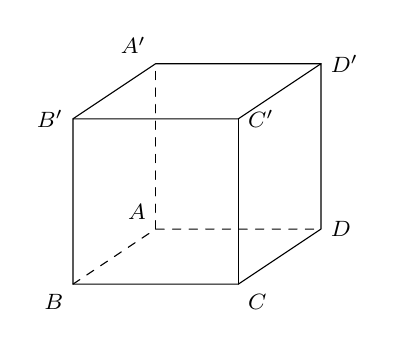
\begin{tikzpicture}[scale=0.7, font=\footnotesize, line join=round, line cap=round, >=stealth]
			\coordinate (B) at (0,0);
			\coordinate (C) at (3,0);
			\coordinate (A) at (1.5,1);
			\coordinate (D) at (4.5,1);
			\coordinate (B') at (0,3);
			\coordinate (C') at (3,3);
			\coordinate (A') at (1.5,4);
			\coordinate (D') at (4.5,4);
			\draw (B) node[below left] {$B$} -- (C) node[below right] {$C$} -- (D) node[right] {$D$} -- (D') node[right] {$D'$} -- (C') node[right] {$C'$} -- (B') node[left] {$B'$} -- cycle;
			\draw (C) -- (C');
			\draw[dashed] (B) -- (A) node[above left] {$A$} -- (D);
			\draw[dashed] (A) -- (A') node[above left] {$A'$};
			\draw (B') -- (A') -- (D');
		\end{tikzpicture}
	}
	\loigiai{
		Vì $ABCD.A'B'C'D'$ là hình hộp chữ nhật nên tứ giác $ABCD$ là hình chữ nhật.\\
		Suy ra hai đoạn thẳng $AD$ và $BC$ song song và bằng nhau, đồng thời $\overrightarrow{AD}$ và $\overrightarrow{BC}$ cùng hướng.\\
		Do đó $\overrightarrow{AD}=\overrightarrow{BC}$.
	}
\end{ex}

\begin{ex}% Câu 10%[Võ Xuân Cường Thịnh]%[1H8N2-2]
	\immini{
		Cho hình chóp $S.ABCD$ có đáy $ABCD$ là hình chữ nhật và $SA \perp (ABCD)$. Đường thẳng nào sau đây vuông góc với mặt phẳng $(SAD)$?
		\choice
		{$BC$}
		{$SB$}
		{$SC$}
		{\True $CD$}
	}{
		\begin{tikzpicture}[scale=0.7, font=\footnotesize, line join=round, line cap=round, >=stealth]
			\coordinate (A) at (1.5,1);
			\coordinate (B) at (0,0);
			\coordinate (C) at (4,0);
			\coordinate (D) at (5.5,1);
			\coordinate (S) at (1.5,4);
			\draw (S) node[above] {$S$} -- (B) node[below left] {$B$} -- (C) node[below right] {$C$} -- (D) node[right] {$D$} -- cycle;
			\draw (S) -- (C);
			\draw[dashed] (S) -- (A) node[below left] {$A$} -- (B);
			\draw[dashed] (A) -- (D);
			\draw pic[draw, angle radius=2mm] {right angle=S--A--D};
			\draw pic[draw, angle radius=2mm] {right angle=S--A--B};
		\end{tikzpicture}
	}
	\loigiai{
		Vì $ABCD$ là hình chữ nhật nên ta có $CD \perp AD$.\\
		Lại có $SA \perp (ABCD)$ nên $CD \perp SA$.\\
		Suy ra $CD \perp (SAD)$.
	}
\end{ex}

\begin{ex}% Câu 11%[Võ Xuân Cường Thịnh]%[2H5N1-1]
	Trong không gian với hệ trục tọa độ $Oxyz$, cho mặt phẳng $(P)$ có phương trình $3(x-2)+2(y-2)-4(z+3)=0$. Điểm nào sau đây thuộc mặt phẳng $(P)$?
	\choice
	{$Q(-2;-3;4)$}
	{$N(-2;-2;3)$}
	{\True $M(2;2;-3)$}
	{$P(3;2;-4)$}
	\loigiai{
		Thay lần lượt tọa độ các điểm ở các đáp án vào vế trái phương trình mặt phẳng $(P)$, ta thấy với điểm $M(2;2;-3)$:
		$$3(2-2)+2(2-2)-4(-3+3) = 3 \cdot 0 + 2 \cdot 0 - 4 \cdot 0 = 0.$$
		Vậy điểm $M(2;2;-3)$ thuộc mặt phẳng $(P)$.
	}
\end{ex}

\begin{ex}% Câu 12%[Võ Xuân Cường Thịnh]%[1D2N2-4]
	Cho cấp số cộng $(u_{n})$ với $u_{1}=1$ và công sai $d=-2$. Giá trị của $u_{3}$ bằng
	\choice
	{$4$}
	{$-5$}
	{$-8$}
	{\True $-3$}
	\loigiai{
		Số hạng tổng quát của cấp số cộng được tính bởi công thức $u_n = u_1 + (n-1)d$.\\
		Áp dụng công thức với $n=3$, $u_1=1$ và $d=-2$, ta có:
		$u_3 = u_1 + 2d = 1 + 2 \cdot (-2) = -3$.
	}
\end{ex}
\Closesolutionfile{ans}

\cauds
\Opensolutionfile{ans}[ans/ans-26-2--SoGD-L1-DS]
\begin{ex}% Câu 1%[Võ Xuân Cường Thịnh]%[1H8V5-6]
	\immini{
		Trong một nhà máy thông minh, hệ tọa độ $Oxyz$ được thiết lập để điều hành các thiết bị tự động, đơn vị trên mỗi trục tọa độ là mét. Mặt sàn nhà máy nằm trên mặt phẳng $(Oxy)$. Một bộ định tuyến phát sóng Wi-Fi được treo tại vị trí $A(-3;4;9)$, một cảm biến đo chấn động được gắn ngầm dưới nền nhà máy tại vị trí $B(6;16;-4)$. Gọi $H$ là hình chiếu vuông góc của $A$ trên mặt sàn. Một robot tự hành $M$ di chuyển trên mặt sàn và luôn giữ khoảng cách đến bộ định tuyến $A$ bằng $15$ m. Biết rằng robot $M$ có nhiệm vụ đồng bộ dữ liệu với cảm biến $B$ và quá trình này đạt độ ổn định cao nhất khi khoảng cách giữa robot và cảm biến là nhỏ nhất.
	}{
		\begin{tikzpicture}[scale=0.8, font=\footnotesize, line join=round, line cap=round, >=stealth]
			% Mặt phẳng (Oxy)
			\draw (-3,-1.5) -- (3,-1.5) -- (5,2) -- (-1,2) -- cycle;
			\node at (4,1.5) {$(Oxy)$};
			% Các điểm
			\coordinate (H) at (0,0);
			\coordinate (A) at (0,3.5);
			\coordinate (B) at (1,-2.5);
			\coordinate (M) at (1.8, -0.6); 
			% Vẽ các đường nối
			\draw[dashed] (A) -- (H);
			\draw (A) -- (M);
			\draw (M) -- (B);
			\draw[dashed] (H) -- (M);
			% Ký hiệu góc vuông
			\draw pic[draw, angle radius=2mm] {right angle=A--H--M};
			% Đánh dấu điểm và nhãn
			\fill (A) circle (1.5pt) node[above] {$A$};
			\fill (H) circle (1.5pt) node[below left] {$H$};
			\fill (B) circle (1.5pt) node[below right] {$B$};
			\fill (M) circle (1.5pt) node[right] {$M$};
		\end{tikzpicture}
	}
	\choiceTF
	{\True Điểm $H$ có tọa độ là $(-3;4;0)$}
	{Khoảng cách từ cảm biến $B$ đến mặt sàn nhà máy là $5$ m}
	{\True Trong quá trình di chuyển, khoảng cách từ robot $M$ đến điểm $H$ luôn không đổi và bằng $12$ m}
	{Khi quá trình đồng bộ dữ liệu đạt độ ổn định cao nhất, khoảng cách giữa robot $M$ và cảm biến $B$ là $6$ m}
	\loigiai{
		\begin{center}
			\begin{tikzpicture}[scale=0.8, font=\footnotesize, line join=round, line cap=round, >=stealth]
				% Mặt phẳng (Oxy)
				\draw (-3,-1.5) -- (3,-1.5) -- (5,2) -- (-1,2) -- cycle;
				\node at (4,1.5) {$(Oxy)$};
				% Các điểm
				\coordinate (H) at (0,0);
				\coordinate (A) at (0,3.5);
				\coordinate (B) at (1,-2.5);
				\coordinate (B') at (1,-1.4);
				\coordinate (M) at (1.8, -0.6); 
				% Vẽ các đường nối
				\draw[dashed] (A) -- (H);
				\draw (A) -- (M);
				\draw (M) -- (B);
				\draw[dashed] (H) -- (M);
				% Ký hiệu góc vuông
				\draw pic[draw, angle radius=2mm] {right angle=A--H--M};
				% Đánh dấu điểm và nhãn
				\fill (A) circle (1.5pt) node[above] {$A$};
				\fill (H) circle (1.5pt) node[below left] {$H$};
				\fill (B) circle (1.5pt) node[below right] {$B$};
				\fill (B') circle (1.5pt) node[above left] {$B'$};
				\fill (M) circle (1.5pt) node[right] {$M$};
			\end{tikzpicture}
		\end{center}
		\begin{itemchoice}
			\itemch Vì mặt sàn nhà máy nằm trên mặt phẳng $(Oxy)$ (có phương trình $z=0$) nên hình chiếu vuông góc $H$ của điểm $A(-3;4;9)$ lên mặt sàn có tọa độ là $H(-3;4;0)$.
			\itemch Khoảng cách từ cảm biến $B(6;16;-4)$ đến mặt sàn $(Oxy)$ là
			$$\mathrm{d}\left(B, (Oxy)\right) = |-4| = 4\ m.$$
			\itemch Robot $M$ di chuyển trên mặt sàn $(Oxy)$ nên toạ độ điểm $M(x;y;0)$. Theo giả thiết, ta có $AM = 15$.\\
			Xét tam giác $AHM$ vuông tại $H$ (do $AH \perp (Oxy)$), áp dụng định lý Pythagore ta có
			$$HM = \sqrt{AM^2 - AH^2} = \sqrt{15^2 - 9^2} = \sqrt{225 - 81} = \sqrt{144} = 12 (\mathrm{m}).$$
			Vậy quỹ đạo của robot $M$ là đường tròn $(C)$ tâm $H$, bán kính $R=12$ trên mặt phẳng $(Oxy)$.
			\itemch Quá trình đồng bộ đạt độ ổn định cao nhất khi khoảng cách $MB$ nhỏ nhất.\\
			Gọi $B'$ là hình chiếu vuông góc của $B(6;16;-4)$ lên $(Oxy)$, ta có $B'(6;16;0)$ và $BB' = 4$.\\
			Ta có $MB = \sqrt{MB'^2 + BB'^2} = \sqrt{MB'^2 + 16}$. \\
			Để $MB$ nhỏ nhất thì $MB'$ phải đạt giá trị nhỏ nhất.\\
			Khoảng cách giữa tâm $H$ của đường tròn quỹ đạo và $B'$ là
			$$HB' = \sqrt{(6 - (-3))^2 + (16 - 4)^2} = \sqrt{9^2 + 12^2} = 15.$$
			Vì $HB' = 15 > R = 12$ nên điểm $B'$ nằm ngoài đường tròn $(C)$.\\
			Giá trị nhỏ nhất của $MB'$ là $MB'_{\min} = HB' - R = 15 - 12 = 3$ m.\\
			Suy ra giá trị nhỏ nhất của khoảng cách $MB$ là
			$$MB_{\min} = \sqrt{(MB'_{\min})^2 + 16} = \sqrt{3^2 + 16} = 5(\mathrm{m}).$$ 
		\end{itemchoice}
	}
\end{ex}

\begin{ex}% Câu 2%[Võ Xuân Cường Thịnh]%[2D5H2-4]
	Một cửa hàng có $200$ hạt giống hoa hướng dương và $300$ hạt giống hoa cúc. Tỉ lệ nảy mầm của hạt giống hoa cúc là $90\%$, của hạt giống hoa hướng dương là $80\%$. Một chuyên gia nông nghiệp chọn ngẫu nhiên một hạt giống. Chuyên gia sử dụng máy quét tia X để dự đoán khả năng nảy mầm của hạt giống. Nếu hạt giống có khả năng nảy mầm, máy quét báo \lq\lq Đạt\rq\rq\, với xác suất $90\%$. Nếu hạt giống không có khả năng nảy mầm, máy quét báo \lq\lq Đạt\rq\rq\, với xác suất $10\%$.
	\choiceTF
	{\True Xác suất chuyên gia chọn được hạt giống hoa cúc là $0{,}6$}
	{\True Biết rằng chuyên gia đã chọn được hạt giống hoa cúc, xác suất để hạt giống đó không nảy mầm là $0{,}1$}
	{Xác suất chuyên gia chọn được hạt nảy mầm là $0{,}84$}
	{\True Một hạt giống sau khi quét kiểm tra, máy đã báo \lq\lq Đạt\rq\rq. Xác suất để hạt giống đó thực sự không nảy mầm nhỏ hơn $0{,}02$}
	\loigiai{
		Tổng số hạt giống là $200 + 300 = 500$ hạt.\\
		Ta gọi 
		\begin{itemize}
			\item $A$ là biến cố \lq\lq Hạt giống nảy mầm\rq\rq.
			\item $B$ là biến cố \lq\lq Máy báo Đạt\rq\rq.
			\item $C$ là biến cố \lq\lq Chọn hạt giống hoa cúc\rq\rq.
			\item $D$ là biến cố \lq\lq Chọn hạt giống hướng dương\rq\rq.
		\end{itemize}
		\begin{itemchoice}
			\itemch Xác suất chọn được hạt giống hoa cúc là $\mathrm{P}(D) =\dfrac{300}{500} = 0{,}6$.
			\itemch Tỉ lệ nảy mầm của hoa cúc là $90\%$ nên xác suất để hạt giống hoa cúc không nảy mầm là 
			$$\mathrm{P}(\overline{C}) = 1 - \mathrm{P}(C) = 100\% - 90\% = 10\% = 0{,}1.$$
			\itemch Xác suất chọn được hạt giống hoa hướng dương là $\mathrm{P}(D) = \dfrac{200}{500} = 0{,}4$.\\
			Xác suất chọn được hạt nảy mầm là 
			$$P(A) = \mathrm{P}(C)\cdot\mathrm{P}(A\mid C) + \mathrm{P}(D)\cdot\mathrm{P}(A\mid D) =  0{,}6 \cdot 0{,}9 + 0{,}4 \cdot 0{,}8 = 0{,}54 + 0{,}32 = 0{,}86 \ne 0{,}84.$$
			\itemch 
			Ta có $\mathrm{P}(A) = 0{,}86$, suy ra xác suất hạt không nảy mầm là $P(\overline{A}) = 1 - 0{,}86 = 0{,}14$.\\
			Xác suất máy báo Đạt là
			$$\mathrm{P}(B) = \mathrm{P}(A) \cdot \mathrm{P}(B|A) + \mathrm{P}(\overline{A}) \cdot \mathrm{P}(B|\overline{A}) = 0{,}86 \cdot 0{,}9 + 0{,}14 \cdot 0{,}1 = 0{,}774 + 0{,}014 = 0{,}788.$$
			Xác suất để hạt giống thực sự không nảy mầm khi máy đã báo Đạt là
			\[ \mathrm{P}(\overline{A}|B) = \dfrac{\mathrm{P}(\overline{A} \cap B)}{\mathrm{P}(B)} = \dfrac{0{,}14 \cdot 0{,}1}{0{,}788} = \dfrac{0{,}014}{0{,}788} \approx 0{,}0177 < 0{,}02. \]
		\end{itemchoice}
	}
\end{ex}

\begin{ex}% Câu 3%[Võ Xuân Cường Thịnh]%[2D1H2-2]
	Cho hàm số $f(x)=x^3-3x+1$.
	\choiceTF
	{Đạo hàm của hàm số đã cho là $f'(x)=3x^2-2$}
	{\True Phương trình $f'(x)=0$ có tập nghiệm là $S=\{-1; 1\}$}
	{\True Ta có $f(1)=-1$, $f(-1)=3$}
	{Gọi $f_{\text{CĐ}}$, $f_{\text{CT}}$ lần lượt là giá trị cực đại và giá trị cực tiểu của hàm số đã cho. Khi đó $f_{\text{CĐ}}-f_{\text{CT}}=3$}
	\loigiai{
		\begin{itemchoice}
			\itemch Ta có $f'(x) = 3x^2 - 3$.
			\itemch Ta có
			\begin{eqnarray*}
				 f'(x) = 0 &\Leftrightarrow& 3x^2 - 3 = 0 \\
				 &\Leftrightarrow& x^2 = 1 \\
				 &\Leftrightarrow & x = \pm 1.
			\end{eqnarray*}
			 Tập nghiệm $S=\{-1; 1\}$.
			\itemch 
			\begin{itemize}
			\item $f(1) = 1^3 - 3 \cdot 1 + 1 = -1$.
			\item $f(-1) = (-1)^3 - 3 \cdot (-1) + 1 = 3$.
			\end{itemize}
			\itemch 
			Bảng biến thiên
			\begin{center}
				
\begin{tikzpicture}
					\tkzTabInit[nocadre=false,lgt=1.2,espcl=3,deltacl=0.6]
					{$x$ /1.2, $y'$ /1.2, $y$ /2.5}
					{$-\infty$,$-1$,$1$,$+\infty$}
					\tkzTabLine{,+,$0$,-,$0$,+,}
					\tkzTabVar{-/$-\infty$,+/$3$,-/$-1$,+/$+\infty$}
				\end{tikzpicture}
			\end{center}
			Dựa vào bảng biến thiên, ta thấy hàm số đạt cực đại tại $x=-1$ với $f_{\text{CĐ}} = 3$ và đạt cực tiểu tại $x=1$ với $f_{\text{CT}} = -1$. 
			Do đó $f_{\text{CĐ}} - f_{\text{CT}} = 3 - (-1) = 4 \ne 3$.
		\end{itemchoice}
	}
\end{ex}

\begin{ex}% Câu 4%[Võ Xuân Cường Thịnh]%[2D4V1-6]
	Một nghiên cứu khả năng ghi nhớ kiến thức của người học sau khi kết thúc khóa học chỉ ra rằng càng về lâu thì khả năng ghi nhớ kiến thức càng giảm. Nếu xem $f(t)$ là phần trăm kiến thức người học còn nhớ sau $t$ tháng thì $f'(t)$ thể hiện là tốc độ thay đổi kiến thức của người học. Nghiên cứu cho thấy $f'(t)<0$, điều này thể hiện càng về lâu thì khả năng ghi nhớ kiến thức càng giảm. Độ lớn của $f'(t)$ chính là tốc độ giảm sút kiến thức của người học. Hai bạn Thành và Công cùng tham gia một khóa học. Sau khi kết thúc khóa học, phần trăm kiến thức bạn Thành còn nhớ sau $t$ tháng được mô hình hóa bởi hàm số $f(t)=94-12\ln(3t+1)$, với $0\le t\le 24$.
	\choiceTF
	{\True Tại thời điểm khóa học vừa kết thúc, bạn Thành nhớ được $94\%$ kiến thức}
	{Tốc độ thay đổi kiến thức của bạn Thành ở thời điểm sau $t$ tháng kết thúc khóa học là $f'(t)=-\dfrac{12}{3t+1}$}
	{Tại thời điểm sau $3$ tháng khóa học kết thúc, tốc độ giảm sút kiến thức của bạn Thành là $1{,}2\%$/tháng}
	{\True Biết rằng tại mọi thời điểm, tốc độ thay đổi kiến thức của bạn Thành luôn gấp $3$ lần tốc độ thay đổi kiến thức của bạn Công. Tại thời điểm kết thúc khóa học, bạn Công nhớ được $96\%$ kiến thức. Sau $3$ tháng, lượng kiến thức bạn Công còn nhớ được hơn $85\%$}
	\loigiai{
		\begin{itemchoice}
			\itemch Tại thời điểm vừa kết thúc khóa học ($t=0$), ta có $f(0) = 94 - 12\ln(1) = 94\%$.
			\itemch Tốc độ thay đổi kiến thức là $f'(t) = -12 \cdot \dfrac{(3t+1)'}{3t+1} = -\dfrac{36}{3t+1}$.
			\itemch Tại thời điểm $t=3$, tốc độ giảm sút (độ lớn của đạo hàm) là 
			\[|f'(3)| = \left| -\dfrac{36}{3 \cdot 3 + 1} \right| = \dfrac{36}{10} = 3{,}6\%/\text{tháng}.\]
			\itemch Gọi phần trăm kiến thức của Công là $g(t)$. Ta có $g'(t) = \dfrac{1}{3}f'(t) = -\dfrac{12}{3t+1}$.\\
			Suy ra $g(t) = \displaystyle \int -\dfrac{12}{3t+1} \mathrm{\,d}t = -4\ln(3t+1) + C$.\\
			Tại $t=0$, Công nhớ $96\%$ nên $g(0) = -4\ln(1) + C = 96 \Rightarrow C = 96$.\\
			Suy ra $g(t) = 96 - 4\ln(3t+1)$. \\
			Sau 3 tháng  
			\[g(3) = 96 - 4\ln(10) \approx 96 - 4 \cdot 2{,}302 = 86{,}792\% > 85\%.\]
		\end{itemchoice}
	}
\end{ex}
\Closesolutionfile{ans}

\caukq
\Opensolutionfile{ans}[ans/ans-26-2--SoGD-L1-KQ]
\begin{ex}% Câu 1%[Võ Xuân Cường Thịnh]%[2D1H3-6]
	Trong hóa học động học, đối với một phản ứng hóa học nối tiếp, nồng độ của chất trung gian sinh ra sẽ tăng lên đến một đỉnh điểm rồi giảm dần do bị chuyển hóa thành chất khác. Dựa trên dữ liệu thực nghiệm, sự thay đổi nồng độ của một chất trung gian trong bình phản ứng được mô phỏng bởi hàm số: $C(t)=-2t^3+3t^2+12t$. Trong đó, $C(t)$ là nồng độ chất trung gian (đơn vị: mmol/L) và $t$ là thời gian (đơn vị: phút) tính từ thời điểm bắt đầu phản ứng. Biết rằng mô hình toán học này chỉ áp dụng trong $3$ phút đầu tiên của phản ứng $(0\le t\le 3)$. Để thu hoạch được lượng chất trung gian nhiều nhất, hệ thống tự động cần trích xuất dung dịch ngay tại thời điểm nồng độ của nó đạt mức tối đa. Hỏi sau bao nhiêu phút kể từ khi bắt đầu phản ứng, nồng độ chất trung gian đạt giá trị lớn nhất?
	\shortans[]{2}
	\loigiai{
		Xét hàm số $C(t) = -2t^3 + 3t^2 + 12t$ xác định trên đoạn $[0; 3]$.\\
		Ta có $C'(t) = -6t^2 + 6t + 12$.
		$$C'(t) = 0 \Leftrightarrow -6t^2 + 6t + 12 = 0 \Leftrightarrow \hoac{&t=2 \in [0; 3] \\ &t=-1 \notin [0; 3].}$$
		Ta tính các giá trị
		\begin{itemize}
		\item $C(0) = 0$.
		\item $C(2) = -2(2)^3 + 3(2)^2 + 12(2) = -16 + 12 + 24 = 20$.
		\item $C(3) = -2(3)^3 + 3(3)^2 + 12(3) = -54 + 27 + 36 = 9$.
		\end{itemize}
		Vậy giá trị lớn nhất của nồng độ chất trung gian là $20$ mmol/L, đạt được tại thời điểm $t = 2$ phút.
	}
\end{ex}

\begin{ex}% Câu 2%[Võ Xuân Cường Thịnh]%[2D1V3-6]
	Một công ty khai thác tuyến tàu cao tốc chở khách du lịch từ đất liền ra đảo với khoảng cách $60$ km. Giả sử tàu di chuyển với vận tốc $v$ không đổi trên suốt tuyến đường. Chi phí vận hành cho mỗi giờ hoạt động của tàu bao gồm:
	\begin{itemize}
		\item Chi phí nhiên liệu: $100v^3$ (đồng), với $v$ (km/h) là vận tốc của tàu $(v>0)$.
		\item Chi phí cố định (lương thủy thủ đoàn, khấu hao, bến bãi, \ldots): $4\,000\,000$ đồng.
	\end{itemize}
	Để đảm bảo chất lượng dịch vụ, thời gian di chuyển mỗi chuyến không được vượt quá $1$ giờ $30$ phút. Đồng thời, vì lý do an toàn hàng hải, tàu không được chạy quá $55$ km/h. Tàu có sức chứa tối đa $150$ hành khách và giả sử rằng số lượng khách trên mỗi chuyến đi luôn đạt mức tối đa. Ban giám đốc thiết lập mục tiêu lợi nhuận thu được từ mỗi chuyến đi bằng $25\%$ tổng chi phí vận hành của chuyến đó. Để đạt được mức lợi nhuận này trong điều kiện tàu được vận hành với tổng chi phí thấp nhất, giá vé mỗi hành khách phải trả là bao nhiêu nghìn đồng?
	\shortans[]{130}
	\loigiai{
		Thời gian di chuyển là $t = \dfrac{60}{v}$ (giờ).\\
		Theo đề bài, thời gian không vượt quá $1$ giờ $30$ phút ($1{,}5$ giờ) và vận tốc không quá $55$ km/h, do đó
		$$\heva{&\dfrac{60}{v} \le 1{,}5 \\ &v \le 55} \Leftrightarrow \heva{&v \ge 40 \\ &v \le 55} \Rightarrow v \in [40; 55].$$
		Chi phí vận hành cho $1$ giờ là $C_h = 100v^3 + 4\,000\,000$.\\
		Tổng chi phí cho một chuyến đi là
		$$C(v) = C_h \cdot t = \left( 100v^3 + 4\,000\,000 \right) \dfrac{60}{v} = 6\,000v^2 + \dfrac{240\,000\,000}{v}.$$
		Xét hàm $C(v)$ xác định trên đoạn $[40; 55]$ có\\
		$$C'(v) = 12\,000v - \dfrac{240\,000\,000}{v^2} = \dfrac{12\,000v^3 - 240\,000\,000}{v^2}.$$
		\begin{eqnarray*}
			C'(v) = 0 &\Leftrightarrow& v^3 = 20\,000\\
			 &\Leftrightarrow& v = \sqrt[3]{20\,000} \approx 27{,}14 \notin [40; 55].
		\end{eqnarray*}
		Vì $v \in [40; 55]$ nên $v > 27{,}14 \Rightarrow C'(v) > 0$, tức là hàm số $C(v)$ đồng biến trên đoạn $[40; 55]$.\\
		Do đó, tổng chi phí thấp nhất đạt được khi $v = 40$ km/h.\\
		Tổng chi phí thấp nhất là
		 $$C(40) = 6\,000\cdot 40^2 + \dfrac{240\,000\,000}{40} = 9\,600\,000 + 6\,000\,000 = 15\,600\,000\,  \text{(đồng)}.$$
		Lợi nhuận mục tiêu là $25\%$ tổng chi phí, nên tổng doanh thu thu về phải bằng $125\%$ tổng chi phí
		$$1{,}25 \cdot 1\,600\,000 = 19\,500\,000\, \text{(đồng)}.$$
		Mỗi chuyến có $150$ hành khách, vậy giá vé mỗi hành khách phải trả là
		$\dfrac{19\,500\,000}{150} = 130\,000$ (đồng).
	}
\end{ex}

\begin{ex}%Câu 3%[Võ Xuân Cường Thịnh]%[2D4V3-1]
\immini{	Trong một mô hình kinh tế, hàm cung $y=S(x)$ là giá của một sản phẩm khi nhà sản xuất sẵn sàng bán ra $x$ sản phẩm, hàm cầu $y=D(x)$ là giá của một sản phẩm khi người tiêu dùng có nhu cầu mua $x$ sản phẩm. Điểm cắt nhau $(x_0; y_0)$ của đồ thị hàm cầu và hàm cung được gọi là điểm cân bằng thị trường. Các nhà kinh tế gọi thặng dư tiêu dùng là diện tích của hình giới hạn bởi đồ thị hàm cầu, đường ngang $y=y_0$ và trục tung. Tương tự, thặng dư sản xuất là diện tích của hình giới hạn bởi đồ thị của hàm cung, đường ngang $y=y_0$ và trục tung (Hình vẽ).}
{\begin{tikzpicture}[scale=1, font=\scriptsize, line join=round, line cap=round, >=stealth]
		
		% Định nghĩa các hàm số để vẽ và tô màu
		\def\dem{\x, {10/(\x+2)}} % Hàm cầu
		\def\sup{\x, {0.1*\x*\x + 1.1}} % Hàm cung
		
		% Tô màu Thặng dư tiêu dùng (màu xanh nhạt)
		\fill[cyan!15] (0,2) -- (3,2) -- plot[domain=3:0] (\dem) -- (0,5);
		
		% Tô màu Thặng dư sản xuất (màu hồng nhạt)
		\fill[magenta!15] (0,2) -- (0,1.1)-- plot[domain=0:3] (\sup) -- (3,2) -- cycle;
		
		% Vẽ hệ trục tọa độ
		\draw[->, thick] (-0.7, 0) -- (6.5, 0) node[below] {$x$};
		\draw[->, thick] (0, -0.7) -- (0, 5.5) node[left] {$y$};
		\node[below left, text=cyan] at (0,0) {O};
		
		% Vẽ đồ thị Hàm cầu và Hàm cung
		\draw[cyan, thick, smooth, domain=0:6] plot (\dem);
		\draw[cyan, thick, smooth, domain=0:6] plot (\sup);
		
		% Các đường gióng đứt nét và Điểm cân bằng
		\draw[dashed, magenta, thick] (3,0) node[below, text=black] {$x_0$} -- (3,2) -- (0,2) node[left, text=black] {$y_0$};
		\fill (3,2) circle (1.5pt);
		\node[right] at (3.2, 2) {$(x_0; y_0)$};
		
		% Chữ bên trong vùng tô màu
		\node[right, align=left] at (0.1, 2.5) {Thặng dư\\tiêu dùng};
		\node[right, align=left] at (0.1, 1.6) {Thặng dư\\sản xuất};
		
		% Chú thích Điểm cân bằng
		\draw (3,2) --++ (100:0.5) node [above] {Điểm cân bằng};
		
		% Hộp thoại chú thích Hàm cầu
		\node[fill=cyan!30, inner sep=4pt] (HC) at (1.5, 4.8) {Hàm cầu};
		\fill[cyan!30] ([xshift=-12pt]HC.south) -- (0.8, 3.5) -- ([xshift=0pt]HC.south) -- cycle;
		
		% Hộp thoại chú thích Hàm cung
		\node[fill=cyan!30, inner sep=4pt] (HCung) at (1.5, -0.8) {Hàm cung};
		\fill[cyan!30] ([xshift=-12pt]HCung.north) -- (0.5, 1.12) -- ([xshift=0pt]HCung.north) -- cycle;
		
\end{tikzpicture}}
	Xem xét thị trường tấm pin năng lượng mặt trời thế hệ mới được mô hình hóa theo mô hình kinh tế này. Hàm cầu là $p=D(x)=4-0{,}2x$ (triệu đồng/tấm). Hàm cung là $p=S(x)=0{,}4+0{,}1x+\dfrac{1}{m}x^2$ (triệu đồng/tấm). Trong đó $x$ là sản lượng (đơn vị: nghìn sản phẩm), $p$ là giá bán (đơn vị: triệu đồng/sản phẩm) và $m$ là chỉ số hiệu quả công nghệ ($m>0$). Biết rằng tại trạng thái cân bằng thị trường, thặng dư sản xuất đạt được là $4{,}2$ tỷ đồng. Tại thời điểm này, thặng dư tiêu dùng là bao nhiêu tỷ đồng?
	\shortans[]{0{,}4}
	\loigiai{
	Do $x$ tính bằng nghìn sản phẩm, $p$ tính bằng triệu đồng/sản phẩm nên một đơn vị diện tích trên hệ tọa độ $Oxy$ tương ứng với $10^3 \cdot 10^6 = 10^9$ đồng $= 1$ tỷ đồng.\\
	Tại trạng thái cân bằng thị trường $(x_0; y_0)$, ta có $D(x_0) = S(x_0) = y_0$, suy ra
	\[ 4 - 0{,}2x_0 = 0{,}4 + 0{,}1x_0 + \dfrac{1}{m}x_0^2 \Leftrightarrow \dfrac{1}{m}x_0^2 = 3{,}6 - 0{,}3x_0. \]
	Thặng dư sản xuất đạt $4{,}2$ tỷ đồng, nên ta có phương trình
	\allowdisplaybreaks
	\begin{eqnarray*}
		&& \int \limits_0^{x_0} \big[ y_0 - S(x) \big] \mathrm{d}x = 4{,}2 \notag \\
		&\Leftrightarrow & \int \limits_0^{x_0} \left[ 4 - 0{,}2x_0 - \left( 0{,}4 + 0{,}1x + \dfrac{1}{m}x^2 \right) \right] \mathrm{d}x = 4{,}2 \notag \\
		&\Leftrightarrow & (3{,}6 - 0{,}2x_0)x - 0{,}05x^2 - \dfrac{1}{3m}x^3 \Big|_0^{x_0} = 4{,}2 \notag \\
		&\Leftrightarrow & 3{,}6x_0 - 0{,}2x_0^2 - 0{,}05x_0^2 - \dfrac{1}{3}\cdot\left( \dfrac{1}{m}x_0^2 \right)x_0 = 4{,}2 \notag \\
		&\Leftrightarrow & 3{,}6x_0 - 0{,}25x_0^2 - \dfrac{1}{3}(3{,}6 - 0{,}3x_0)x_0 = 4{,}2 \notag \\
		&\Leftrightarrow & 3{,}6x_0 - 0{,}25x_0^2 - 1{,}2x_0 + 0{,}1x_0^2 = 4{,}2 \notag \\
		&\Leftrightarrow & -0{,}15x_0^2 + 2{,}4x_0 - 4{,}2 = 0 \\
		&\Leftrightarrow& \hoac{&x_0 = 14 \\ &x_0 = 2.}
	\end{eqnarray*}
	Ta có
	\begin{itemize}
	\item Với $x_0 = 14$, ta có $\dfrac{1}{m} \cdot 14^2 = 3{,}6 - 0{,}3 \cdot 14 = -0{,}6 < 0$ (loại vì $m > 0$).
	\item Với $x_0 = 2$, ta có $\dfrac{1}{m} \cdot 2^2 = 3{,}6 - 0{,}3 \cdot 2 = 3 > 0 \Rightarrow m = \dfrac{4}{3}$ (nhận).
	\end{itemize}
	
	Khi $x_0 = 2$, giá cân bằng là $y_0 = 4 - 0{,}2 \cdot 2 = 3{,}6$.
	Thặng dư tiêu dùng là
	\[ \int \limits_0^2 [D(x) - y_0] \mathrm{d}x = \int \limits_0^2 (4 - 0{,}2x - 3{,}6) \mathrm{\,d}x = \int \limits_0^2 (0{,}4 - 0{,}2x) \mathrm{\,d}x =  0{,}4x - 0{,}1x^2 \Big|_0^2 = 0{,}4. \]
	Vậy tại thời điểm này, thặng dư tiêu dùng là $0{,}4$ tỷ đồng.
	}
\end{ex}

\begin{ex}%Câu 4%[Võ Xuân Cường Thịnh]%[0D8C2-5]
	Một máy chủ cần xử lý tuần tự $15$ tệp dữ liệu khác nhau, bao gồm: $3$ tệp văn bản, $5$ tệp âm thanh và $7$ tệp video. Việc xử lý liên tục các tệp dữ liệu cùng loại sẽ làm giảm hiệu suất của hệ thống. Do đó, hệ thống phải sắp xếp thứ tự xử lý sao cho không có bất kỳ hai tệp dữ liệu cùng loại nào (văn bản, âm thanh, video) được xếp liền kề nhau. Gọi $S$ là số cách sắp xếp thỏa mãn yêu cầu trên. Hãy tính tổng các chữ số của $S$.
	\shortans[]{36}
	\loigiai{
	Yêu cầu bài toán là xếp $15$ tệp phân biệt thành một hàng ngang sao cho không có $2$ tệp cùng loại nào đứng cạnh nhau.\\
	Xếp $7$ tệp video vào hàng. Để không có $2$ tệp video nào liền kề, ta phải chèn các tệp khác vào $8$ khoảng trống (gồm $6$ khoảng trống ở giữa và $2$ khoảng ở hai đầu).
	\begin{center}
		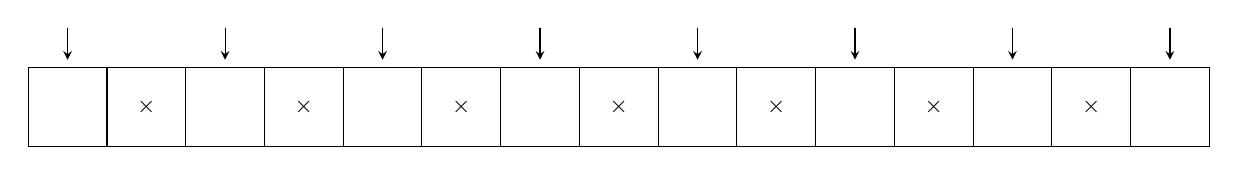
\begin{tikzpicture}[scale=1,>=stealth, font=\footnotesize, line join=round, line cap=round]
			\foreach \x in {0,1,...,15}{
				\draw (\x,-0.5) -- (\x,0.5);
			}
			\foreach \x in {1.5,3.5,5.5,...,14.5}{
			\node at (\x,0) {$\times$};
			}
			\foreach \x in {0.5,2.5,4.5,...,15.5}{
				\draw[->] (\x,1) -- (\x,0.6);
			}
			\draw (0,-0.5) rectangle (15,0.5);
		\end{tikzpicture}
	\end{center}
	Gọi $x_i$ ($i=1, 2, \ldots, 8$) là số lượng tệp được chèn vào khoảng trống thứ $i$.\\
	Ta có $x_2, \ldots, x_7 \ge 1$ và tổng số tệp chèn là $3 + 5 = 8$. 
	\begin{itemize}
	\item Trường hợp 1: Mỗi khoảng chứa đúng $1$ tệp\\
	Ta có $\mathrm{C}_8^3 = 56$ cách chọn vị trí cho văn bản và âm thanh. 
	\item Trường hợp 2: Một khoảng chứa 2 tệp, sáu khoảng chứa 1 tệp, một khoảng ngoài cùng trống
	 \begin{itemize}
	 	\item Chọn $1$ vị trí ngoài cùng trống có $\mathrm{C}^1_2 = 2$ cách; \item Chọn $1$ khoảng trong các khoảng còn lại chứa $2$ tệp có $\mathrm{C}^1_7 = 7$ cách. Cụm $2$ tệp phải là dạng \lq\lq văn bản - âm thanh\rq\rq\, hoặc ngược lại nên có $2$ cách chọn.
	 	\item  Xếp các tệp còn lại vào $6$ vị trí đơn có $\mathrm{C}_6^2 = 15$ cách.
	 \end{itemize} 
	 Tổng cộng có $2 \cdot 7 \cdot 2 \cdot 15 = 420$ cách.
	\item Trường hợp 3: Cả hai vị trí ngoài cùng đều trống, $8$ tệp phân bố vào $6$ khoảng giữa.
	 \begin{itemize}
	 	\item Cách 1: Chọn $2$ khoảng chứa $2$ tệp có $\mathrm{C}_6^2 = 15$ cách. \\
	 	Các cụm đều có $2$ kiểu xếp (VB-AT hoặc AT-VB) $\Rightarrow 2 \cdot 2 = 4$ cách.\\
	 	 Xếp các tệp lẻ còn lại vào $4$ vị trí $\Rightarrow \mathrm{C}_4^1 = 4$ cách. \\
	 	 Do đó có $15 \cdot 4 \cdot 4 = 240$ cách. 
	 	 \item Cách 2: Chọn $1$ khoảng chứa cụm $3$ tệp có $\mathrm{C}^1_6 = 6$ cách.\\
	 	 Nếu cụm này có dạng 
	 	 \begin{itemize}
	 	 	\item VB-AT-VB ta chọn $1$ vị trí cho $1$ tệp VB có $5$ cách.
	 	 	\item  AT-VB-AT ta chọn $2$ vị trí cho 2 tệp VB có $\mathrm{C}^2_5=10$ cách.
	 	 \end{itemize}
	 	 Do đó có $6 \cdot (5 + 10) = 90$ cách.
	\end{itemize}
\end{itemize}
	Suy ra có $56 + 420 + 330 = 806$ cách xếp.
	Hoán vị cách vị trí các tệp mỗi loại ta có 
	\[ S = 806 \cdot 3! \cdot 5! \cdot 7! = 2\,924\,812\,800\, \text{(cách)}. \]
	Tổng các chữ số của $S$ là $2 + 9 + 2 + 4 + 8 + 1 + 2 + 8 + 0 + 0 = 36$.
	}
\end{ex}

\begin{ex}%Câu 5%[Võ Xuân Cường Thịnh]%[2H2V2-6]
	Trong không gian $Oxyz$, mỗi đơn vị trên các trục tọa độ ứng với $1$ mét. Mặt phẳng $(Oxy)$ biểu diễn mặt sàn của một gara, trục $Oz$ hướng thẳng đứng lên trên. Một bức tường thẳng đứng trong gara được mô hình hóa bởi mặt phẳng $(E) \colon 6x+8y=55$. Chiếc ô tô đang lùi chậm vào vị trí đỗ theo hướng vectơ $\overrightarrow{v}=(3; 4; 0)$. Ba cảm biến lùi được gắn cố định trên cản sau của ô tô. Tại thời điểm bắt đầu xét, tọa độ của ba cảm biến lần lượt là $A(4{,}57; 0{,}51; 0{,}5)$, $B(3{,}37; 1{,}41; 0{,}5)$, $C(4; 1; 0{,}5)$. Hệ thống phát tín hiệu cảnh báo \lq\lq Bíp\rq\rq\, tại thời điểm đầu tiên có ít nhất một cảm biến cách bức tường $(E)$ không quá $0{,}3$ mét. Gọi $R(a; b; c)$ là tọa độ của cảm biến đầu tiên đạt ngưỡng cảnh báo. Tính $a-b+c$.
	\shortans[]{3{,}1}
	\loigiai{
	Mặt phẳng $(E) \colon 6x+8y-55=0$ có vectơ pháp tuyến $\overrightarrow{n} = (6; 8; 0) = 2\overrightarrow{v}$. \\
	Do đó, hướng lùi của xe vuông góc với mặt phẳng bức tường.\\
	Giả sử xe di chuyển theo vectơ độ dời là $\overrightarrow{u} = t\overrightarrow{v} = (3t; 4t; 0)$ với $t > 0$.
	Tọa độ điểm $M(x; y; z)$ trên xe tại thời điểm $t$ là $M_t(x+3t; y+4t; z)$.\\
	Khoảng cách từ $M_t$ đến mặt phẳng $(E)$ là
	\[ \mathrm{d}\left(M_t, (E)\right) = \dfrac{|6\cdot(x+3t) + 8\cdot(y+4t) - 55|}{\sqrt{6^2 + 8^2}} = \dfrac{|(6x + 8y - 55) + 50t|}{10}. \]
	Đặt $f(M) = 6x + 8y - 55$, ta có
	\begin{itemize}
	\item $f(A) = 6 \cdot 4{,}57 + 8 \cdot 0{,}51 - 55 = -23{,}5$.
	\item $f(B) = 6 \cdot 3{,}37 + 8 \cdot 1{,}41 - 55 = -23{,}5$.
	\item $f(C) = 6 \cdot 4 + 8 \cdot 1 - 55 = -23$.
	\end{itemize}
	Vì $f(M) < 0$ tại các điểm gắn cảm biển nên khi lùi xe giá trị $f(M_t) = f(M) + 50t$ sẽ tăng dần từ số âm về $0$.
	Cảm biến đạt ngưỡng cảnh báo đầu tiên khi
	\[ \mathrm{d}\left(M_t, (E)\right) = 0{,}3 \Leftrightarrow \dfrac{|f(M) + 50t|}{10} = 0{,}3 \Leftrightarrow f(M) + 50t = -3. \]
	Thời điểm đó là $t = \dfrac{-3 - f(M)}{50}$.\\
	Để $t$ nhỏ nhất, $f(M)$ phải lớn nhất. Do $f(C) = -23$ lớn nhất trong ba giá trị nên cảm biến $C$ phát cảnh báo đầu tiên, ứng với $t = \dfrac{-3 - (-23)}{50} = 0{,}4$.\\
	Tọa độ cảm biến $C$ lúc này là
	\[ R = C + 0{,}4\overrightarrow{v} = (4 + 0{,}4 \cdot 3; 1 + 0{,}4 \cdot 4; 0{,}5) = (5{,}2; 2{,}6; 0{,}5). \]
	Ta được $a = 5{,}2$, $b = 2{,}6$, $c = 0{,}5$.\\
	Vậy $a - b + c = 5{,}2 - 2{,}6 + 0{,}5 = 3{,}1$.
	}
\end{ex}

\begin{ex}%Câu 6%[Võ Xuân Cường Thịnh]%[1H8H6-2]
	Cho hình hộp chữ nhật $ABCD.A'B'C'D'$ có đáy $ABCD$ là hình chữ nhật, $AB=4AD=4a$ và $AA'=a$. Gọi $\alpha$ là số đo của góc nhị diện $[A', BD, C]$. Tính $\alpha$ theo đơn vị độ, làm tròn kết quả đến hàng đơn vị.
	\shortans[]{134}
	\loigiai{
		\begin{center}
			\begin{tikzpicture}
				\def\a{3}
				\def\b{2}
				\def\h{3.5}
				\path 	(0:0) coordinate (A)
				++(0:\a) coordinate (D)
				++(-130:\b) coordinate (C)
				($(A)+(C)-(D)$) coordinate (B)
				($(A)+(90:\h)$) coordinate (A')
				($(B)+(90:\h)$) coordinate (B')
				($(C)+(90:\h)$) coordinate (C')
				($(D)+(90:\h)$) coordinate (D')
				($(B)!(A)!(D)$) coordinate (H);
				\draw[dashed,thick] 	(B)--(A)--(D)	(A)--(A') (B)--(D) (A)--(H);
				\draw[thick] 	(C)--(C') 	(D)--(D') 	(B)--(B')	(C)--(C')
				(B)--(C)--(D) 
				(A')--(B')--(C')--(D')--cycle;
				\foreach \x/\g in {A/180,B/180,C/0,D/0,A'/180,B'/180,C'/0,D'/0,H/-20}
				\fill[black] 	(\x) circle (1pt)
				($(\g:4mm)+(\x)$) node {$\x$};	
			\end{tikzpicture}
		\end{center}
	Gọi $H$ là hình chiếu vuông góc của $A$ lên $BD$.\\
	Vì $A'A \perp (ABCD)$ nên $A'A \perp BD$. \\
	Suy ra $BD \perp (A'AH) \Rightarrow BD \perp A'H$.\\
	Từ đó, góc phẳng nhị diện $[A', BD, A]$ chính là $\widehat{A'HA}$.\\
	Xét tam giác $ABD$ vuông tại $A$, có đường cao $AH$
	\[ \dfrac{1}{AH^2} = \dfrac{1}{AB^2} + \dfrac{1}{AD^2} = \dfrac{1}{16a^2} + \dfrac{1}{a^2} = \dfrac{17}{16a^2} \Rightarrow AH = \dfrac{4a}{\sqrt{17}}. \]
	Trong tam giác vuông $A'AH$ tại $A$
	\[ \tan \widehat{A'HA} = \dfrac{A'A}{AH} = \dfrac{a}{\dfrac{4a}{\sqrt{17}}} = \dfrac{\sqrt{17}}{4} \Rightarrow \widehat{A'HA} \approx 45{,}87^\circ. \]
	Mặt khác, trong mặt phẳng đáy $(ABCD)$, điểm $A$ và điểm $C$ nằm ở hai phía đối nhau đối với đường thẳng $BD$. Do đó, hai nửa mặt phẳng bờ $BD$ đi qua $A$ và đi qua $C$ tạo thành một góc $180^\circ$.\\
	Suy ra góc nhị diện $[A', BD, C]$ và góc nhị diện $[A', BD, A]$ là hai góc bù nhau.\\
	Vậy $\alpha = 180^\circ - \widehat{A'HA} \approx 180^\circ - 45{,}87^\circ = 134{,}13^\circ  \approx 123^\circ$.
	}
\end{ex}
\Closesolutionfile{ans}